\chapter{Random Walks}\label{ch:random-walk}

A drunkard leaves his favorite bar and walks to his home. After $N$ steps, how far is he from the bar?  This is a basic question of random walk problems.  An interesting mathematics such as Wiener process evolved from this simple question and many important theories have been developed in many fields of science based on the random walk model.  In this chapter, we focus on discrete random walks where step size is finite and fixed.  Continuous random walk is discussed in Chapter \ref{ch:langevin}.

\section{One-dimensional Random Walk}

\begin{figure}
	\centering
	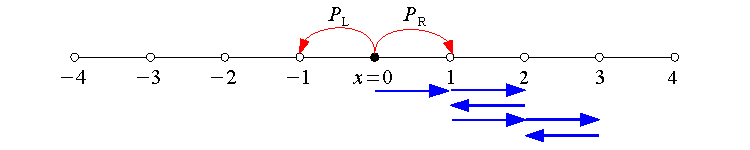
\includegraphics[width=4in]{16.Random-Walk/1d_random_walk.pdf}
	\caption{One-dimensional discrete random walk. The blue arrows indicate a realization of 6-steps trajectory, $RRLRRL$}
	\label{fig:1d_random_walk}
\end{figure}

A particle in a one-dimensional space jumps from one site to an adjacent site at random with a probability $p_L=p$ to the right and $p_R=1-p$ to the left.  See Fig. \ref{fig:1d_random_walk}.  The position of the particle is specified by integer index assigned to the grid point.
We assume $p=\frac{1}{2}$ for now.  Then, we have unbiased random walk ($p_L=p_R$). Initially a particle is placed at $x_0$.  Where is the particle after $N$ steps?  There is no definite answer to this question. The trajectory of the particle is not uniquely determined by the initial condition since the direction of jump is probabilistic.  Therefore, the position of the particle at  time $t$ is stochastic variable $\hat{X}_t$ defined with sample space $x \in \mathbb{Z}$ and probability distribution $P_t(x)$.  Here time, $t=0, 1, \cdots, N$ is just the number of jumps the particle made and thus discrete.   The stochastic variable $\hat{X}_t$ as a function time $t$ is a sequence of random variables
$\{\hat{X}_0, \hat{X}_1, \hat{X}_2, \cdots\}$, which is called stochastic process.
For example, if the particle was initially at $x=0$, the possible outcome is $\{0\}$the probability is $P_0(x)=\delta_{x\,0}$ where $\delta_{m\,n}$ is a Kronecker's delta.  At $t=1$, the particle is either at $x=1$ or $x=-1$.  Thus, the possible outcome is $\{\pm 1\} $ and the associate probability is
\begin{equation}
P_1(x) = 
\begin{cases}
\displaystyle\frac{1}{2} & \text{for  } x=\pm 1 \\[1.5ex]
0 & \text{otherwise}
\end{cases}.
\end{equation}
After the second jumps, the possible outcomes of $\hat{X}_2$ are now $\{-2,0,2\}$ with the probability
\begin{equation}
P_2(x) = 
\begin{cases}
\displaystyle\frac{1}{2} & \text{for  } x=0 \\[1.5ex]
\displaystyle\frac{1}{4} & \text{for  } x=\pm 2 \\[1.5ex]
0 & \text{otherwise}
\end{cases}.
\end{equation}

This problem can be solved analytically for $t=N$.  Suppose that the particle jumps to the right $N_\textsc{R}$  times and to the left $N_\textsc{L}=N-N_\textsc{R}$. (Note that $N=N_\textsc{R}+N_\textsc{L}$.)
For example, the blue arrows in Fig. \ref{fig:1d_random_walk} represents an trajectory of $N=6$ steps of which $N_\textsc{R}=4$ steps to the right and $N_\textsc{L}=2$ to the left. The final position $x(N_\textsc{R},N)=(N_\textsc{R}-N_\textsc{L}) = 2$.  The probability to have this particular trajectory $RRLRRL$ is $\left (\displaystyle \frac{1}{2} \right )^6$.  However, several other trajectories have the same $N_\textsc{R}$ and 
$N_\textsc{L}$, e.g., $RRRRLL$.  Simple combinatorial calculation tells that there are
\begin{equation}
W(N_\textsc{R},N) = \frac{N!}{N_\textsc{R}!\, (N-N_\textsc{R})!}
\end{equation}
different ways to reach the same point. Noting that the final point is $x=(N_\textsc{R}-N_\textsc{L})=(2 N_\textsc{R}-N)$, $N_\textsc{R}=\frac{1}{2} (N+x)$ and $N_\textsc{L}=\frac{1}{2} (N-x)$. Hence, the probability to find the particle at $x$ after $N$ steps is
\begin{equation}\label{eq:RW_dist}
P_\textsc{n}(x) = \frac{N!}{\left (\displaystyle\frac{N+x}{2} \right)!\, \left (\displaystyle\frac{N-x}{2} \right)!} \left ( \frac{1}{2} \right )^N.
\end{equation}
When $N\pm x$ is not an even integer, this result fails. This is because when $N$ is even, the particle cannot stop at any odd site and similarly when $N$ is odd, no even site is reachable by the particle.

When $N \gg 1$, the probability (\ref{eq:RW_dist}) becomes Gaussian\footnote{A special care is needed to make $x$ continuous since $x/a$ is exclusively even or odd.}
\begin{equation}
P_\textsc{n}(x)  \approx \frac{1}{\sqrt{2\pi N}}\me^{-x^2/2N}.
\end{equation}
The mean position is $\expval{X_\textsc{n}}=0$ for any $N$.  The variance increases as $\expval{X_\textsc{n}^2}=N$.  This means that on average the drunkard is still at the bar after a long walk!



\bigskip
\begin{example}

While analytic results of statistical quantities are available for this simple random walk, we often want to see what the individual trajectories look like. Program \ref{prog:rw_1d} simulates simple one-dimensional random walk. The particle is initially at $x=0$. The direction of jump is determined by a standard uniform random number between 0 and 1.  If the random number is less than 0.5, the particle jumps to the left and otherwise to the right.  Repeating it many times, we obtain a trajectory of the particle.  If another particle starts from the same place, its trajectory is different from the first one since the direction of jump is random. In order to evaluate statistical quantities, we need to calculate many trajectories. The program calculates 100000 trajectories.  The mean and variance of the position are computed at each time.  Figure \ref{fig:rw_1d} shows a few individual trajectories, the mean and the square root of variance.  While the mean value remains zero for all time, the individual trajectories do not stay close to the origin and they cover wide area around the origin.  However, roughly speaking,  most trajectories stay inside the square root of the variance.  The distribution of the particles at $t=N$ matches well to the Gaussian distribution.

\begin{figure}
\centering
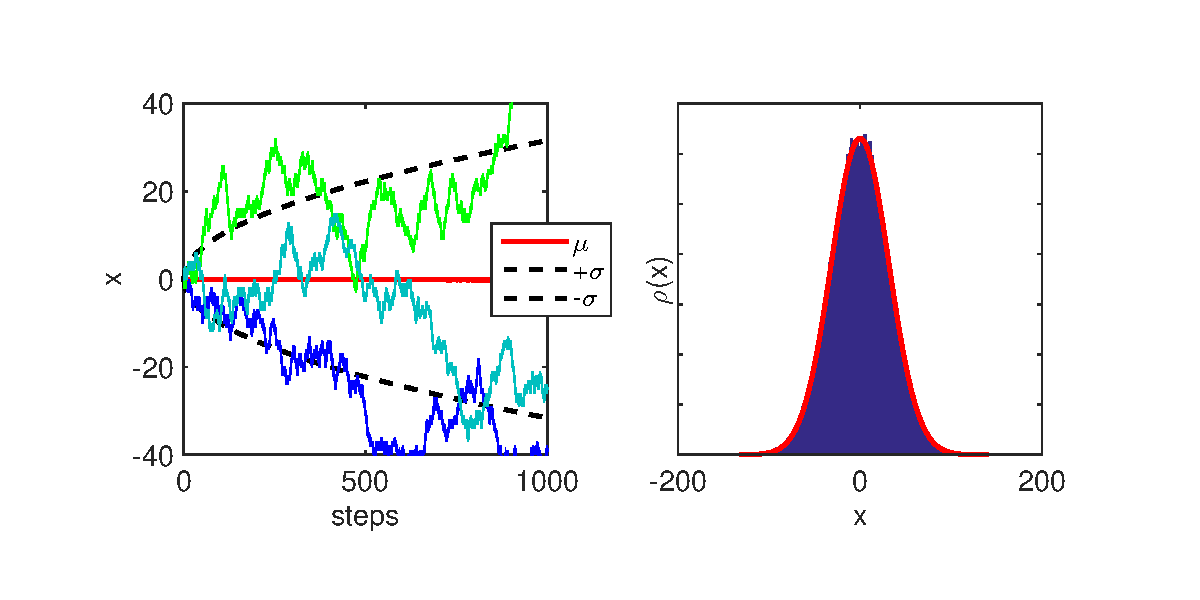
\includegraphics[width=5.0in]{16.Random-Walk/rw_1d.pdf}
\caption{Monte Carlo simulation of discrete random walk.   100000 trajectories are used to get the statistics. Left: The solid and dashed red lines show the mean trajectory and the deviation from the mean. Thin solid lines are individual trajectories.  Right: The distribution at step $N=1000$.  It fits exactly to the Gaussian distribution (red line) with variance $\sigma^2=N$.}
\label{fig:rw_1d}
\end{figure}

\end{example}

\noindent
\section{Persistent Random Walk}

In some random walks, the particles carry inertia such that the jump probability depends on the previous jump.  The particles tend to jump in the same direction as the previous jump but not always.  Such random walk is called persistent random walk.  To simulate it, we introduce a state dependent jump probability.  The particle jumps in the same direction as previous jump with the probability $p>1/2$ and the change the jump direction with the probability $q=1-p$.  This probability does not create a  preferred direction.  Therefore, the mean position remains zero.
However, the variance deviates from that of the normal random walk. Analytical calculation shows that the variance is $\sigma^2=\frac{p}{q}N$. The particle distribution of the persistent random walk is expected to be wider.  We can also use $p<1/2$.  In this cases, the particles tends to jump in the opposite direction to the previous jump ('' Fickle Random Walk'').

\bigskip

\begin{example}

Program \ref{prog:rw_1d_persistent} simulates persistent random walk with $p=0.75$. According to the theory, $\sigma^2 = 3N$ for this case.  Figure \ref{fig:rw_1d_persistent} illustrates that. The $\sigma^2 = 3 N$ in comparison to $\sigma^2 = N$ for the normal random walk.  Try other values of $p$, you will find that $\sigma^2 = N p/q$. Even you can go the other side $p/q<1$ so that the particles tends to change the direction more often than the normal random walk.

\begin{figure}
\centering
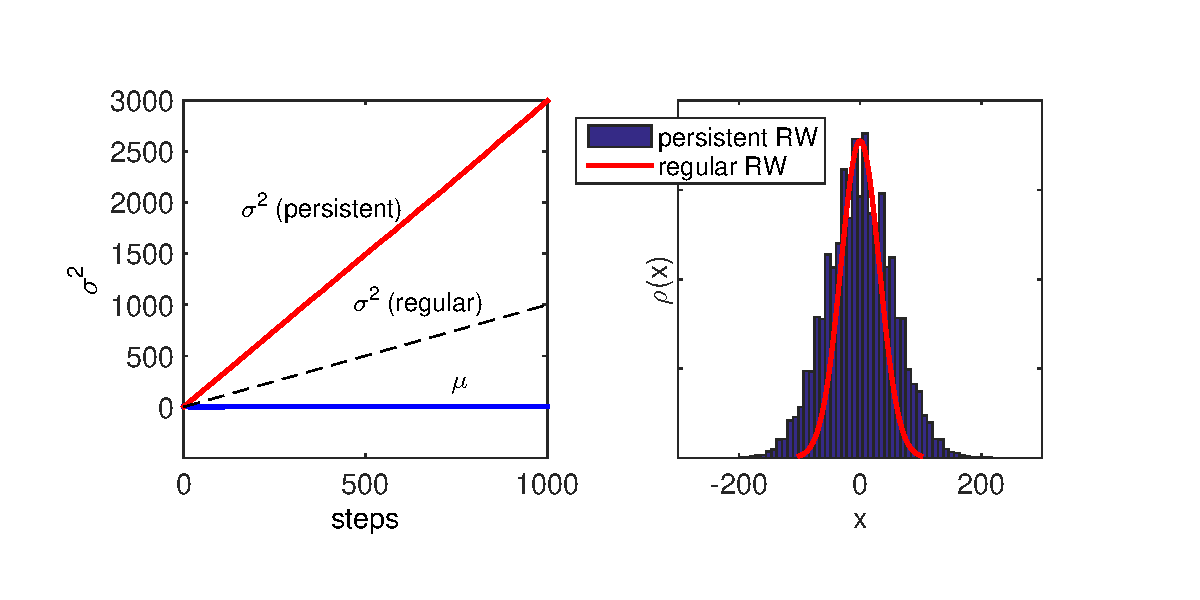
\includegraphics[width=5.0in]{16.Random-Walk/persistent_rw.pdf}
\caption{Simulation of persistent random walk. 100000 trajectories are sampled with a persistent jump probability $p=0.75$.  The left panel shows that the mean position remains zero but the variance grows faster than that of the normal random walk.  The right panel shows the distribution of the particles.  The red line indicates the distribution of the normal random walk (Gaussian).}
\label{fig:rw_1d_persistent}
\end{figure}

\end{example}

\noindent
\section{Multi-dimensional Random Walk}

For $d$-dimensional space, we consider $d$-dimensional cubic lattice.  The random walker jumps to one of the $2d$ nearest sites at random.
If there is no bias, the probability to jump to a particular site is $p=1/2d$.  For the two-dimensional space, there are four possible jumps, east (E), west (W), north (N), and south (S) .  Hence, $p=1/4$.  The final position is
\begin{equation}
x=(N_\textsc{e}-N_\textsc{w}), \qquad y=(N_\textsc{n}-N_\textsc{s})
\end{equation}
and the probability to reach that position after $N$ step is
%
\begin{equation}
P_\textsc{n}(x,y) = \frac{N!}{N_\textsc{E}! N_\textsc{W}! N_\textsc{N}! N_\textsc{S}!} \left(\frac{1}{4}\right )^N, \qquad N_\textsc{R}+N_\textsc{L}+N_\textsc{U}+N_\textsc{D}=N
\end{equation}.
%
The mean position remains at the origin ($\expval{x}=\expval{y}=0$).  The mean square displacement at $N$ steps is
\begin{equation}\label{eq:msd}
\expval{r^2}=\expval{x^2+y^2} = \expval{x^2}+\expval{y^2} = N_x + N_y = N
\end{equation}
where $N_x$ and $N_y$ are the number of steps in $x$ and $y$ direction.  Although $N_x$ and $N_y$ vary but at the mean square displacement only depends on $N$.  

\bigskip
\begin{example}\label{ex:2d-rw}

Program \ref{prog:rw_2d} simulates the two-dimensional random walk with 100,000 particles.
All particles are initially at the origin of the coordinates. Each particle takes a different trajectories from others. Tw independent trajectories are plotted in Fig. \ref{fig:rw_2d_trajectory}.  The radius of the red circle indicates $r$, the square root of the mean square displacement (\ref{eq:msd}).  The final position of the particles are shown in Fig. \ref{fig:rw_2d_distribution}. It is clear that the particle density is higher in the circle.

\begin{figure}
	\centering
	\begin{subfigure}{0.45\textwidth}
		\centering
		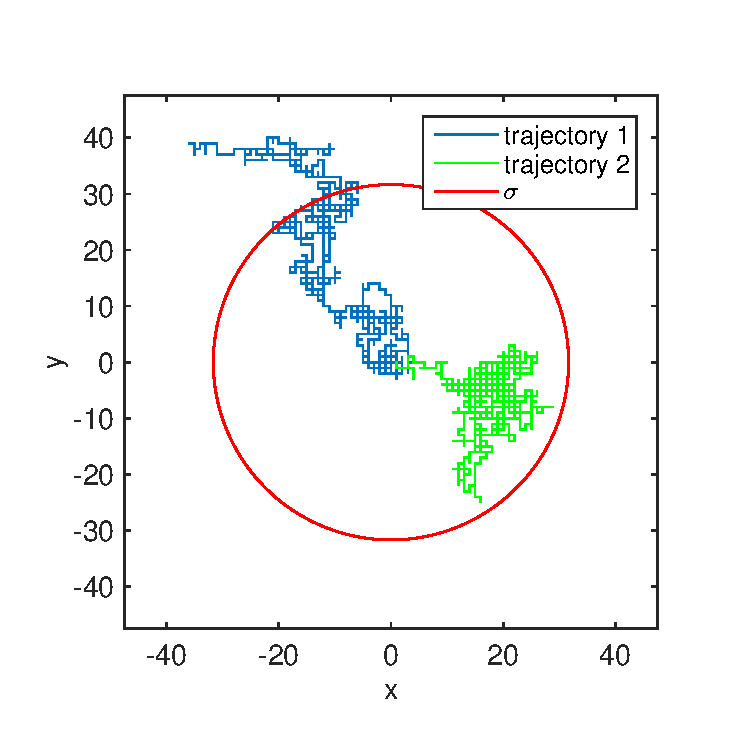
\includegraphics[width=2.5in]{16.Random-Walk/rw_2d_trajectory.pdf}
		\caption{Two independent trajectories (blue and green lines) of two-dimensional discrete random walk ($N=1000$ steps).  The red line indicates the circle of radius $\sigma(N)$.  On average, the random walkers spend most of time inside the circle.}
		\label{fig:rw_2d_trajectory}
	\end{subfigure}
	\begin{subfigure}{0.45\textwidth}
		\centering
		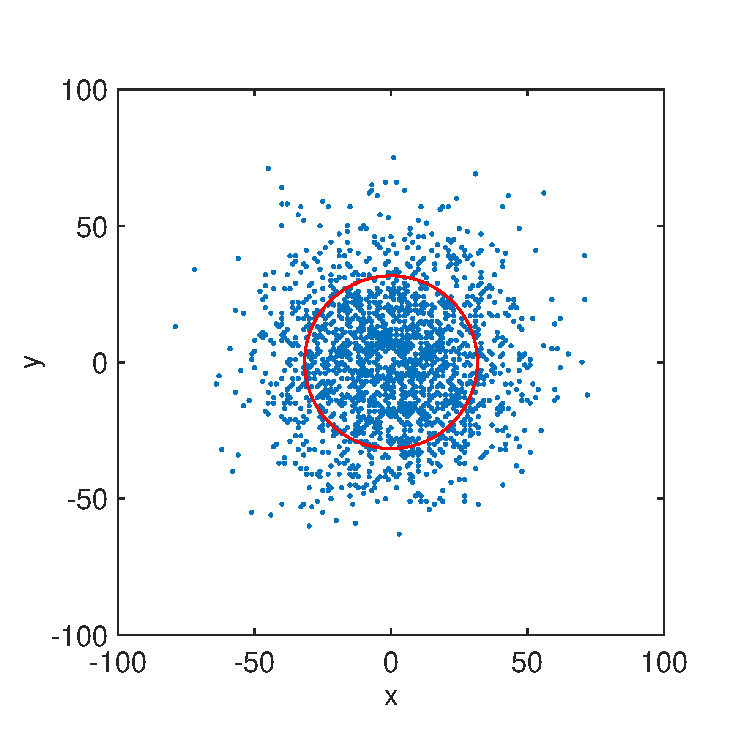
\includegraphics[width=2.5in]{16.Random-Walk/rw_2d_distribution.pdf}
		\caption{The distribution of the particles after $1000$ steps.  $2000$ particles are shown.  The particle density is high inside the red circle.   Many of them are still very close to the starting point.}
		\label{fig:rw_2d_distribution}
	\end{subfigure}
	\caption{Simulation of two-dimensional discrete random walk. Statistics is taken over 100000 trajectories.}\label{fig:rw_2d}
\end{figure}

\end{example}

\noindent
\section{Applications in Physics}

\subsection{Diffusion Limited Aggregates}


Consider mineral ions in solution.  They diffuse randomly and when they hit a surface they stick to it. (See Fig. \ref{fig:deposition_model}.)  Then, the surface grows as more ions arrive.  However, the ions do not fill the space densely as it grows. The ballistic deposition model discussed in the previous chapter is an exmple. Here we discuss another example, the electrodeposition of ions onto a seed particle.  A cluster grown from a copper sulfate solution in an electrodeposition cell is shown in Fig \ref{fig:dla_experiment}.  This type of growth, known as diffusion limited aggregates (DLA), forms a distinct shape with a fractional dimension.\cite{dla}  It turns out that this kind of growth patterns have been observed in other cases such as dendrites grown on a rock. (See next section.)

A mathematical model was developed by Witten and Sander in 1981\cite{dla_theory} based on random walk.  A seed particle is placed at the origin of the coordinates.  Then, a particle is released from a point far from the seed. The particle moves randomly and eventually hits the seed.  Then, it sticks to the seed and forms a cluster.  A second particle is released from a different point again far from the seed. It also travels at random.  Eventually it hits one of the particles in the cluster and sticks to it.  By repeating this procedure the cluster grows.  As the cluster grows, it becomes harder to reach the empty space near the center of the cluster by random walk and thus the empty space remains as the cluster gets bigger. The resulting object in the two-dimensional space is a fractal with a fractional dimension $1<D<2$ where the fractal dimension is determined by the total mass of the object $M$ within a radius $R$ 
\begin{equation}\label{eq:dla-fractal-dimension}
M \propto R^D
\end{equation}
If the whole space inside the circle of radius $R$ is filled with particles or the empty regions are uniformly distributed, then $D=2$.  Figure \ref{fig:dla} indicates that the structure is tree-like. There are many different sizes of branches and empty spaces.  Zooming in, we see a similar structure. It is hard to tell if we zoomed in or not.  Such a kind of structures is said to be self-similar and an important property of a fractal. 

Here we simulate the DLA using discrete random walk.  The two-dimensional space is represented by a square grid.  The particles jump from one site to one of nearest sites at random with equal probability.  The following algorithm is used in Program \ref{fig:dla}.
The resulting aggregate is shown in Fig. \ref{fig:dla_simulation}, which resembles to the cluster generated by the electrodeposition in Fig. \ref{fig:dla}.

\begin{figure}
\centering
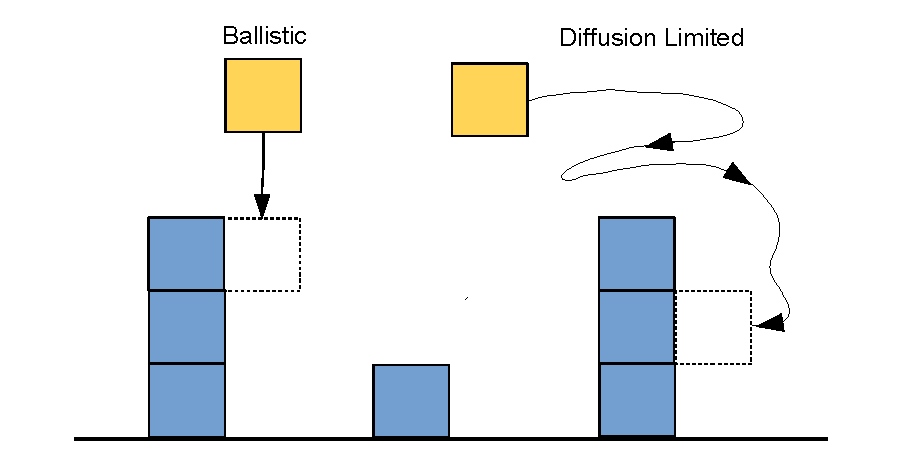
\includegraphics[width=3in]{16.Random-Walk/deposition_model.pdf}
\caption{Two deposition models:  In the ballistic deposition model, the particles do not diffuse.  The lateral position is randomly selected and stick to the first particle in a cluster.  In the diffusion limited model, on the other hand, the particles diffuse laterally as well as vertically.  They stick to the first particle they hit.  Due to the random walk, they can attached to the cluster at any location.} 
\label{fig:deposition_model}
\end{figure}

\begin{myalgobox}
\Algorithm{Two-dimensional Diffusion Limited Aggregates}\label{algo:dla}

\medskip
\begin{minipage}{5.5in}
\small
\begin{enumerate}
\item Place a seed particle at the origin (0,0).
\item Set an initial radius $R$ of the circle where the particles are released.  ($R=5$ was used.)
\item Set an exterior radius $R\text{max}$.  ($R_\text{max}=3R$ is used.  The exterior wall moves out as the cluster gets bigger.)
\item Select a point on a circle at random and release a particle from it.
\item Let the particle undergoes random walk.
\item If the particle reaches $R_\text{max}$, it is lost to the outer wall. Start over again from step 3.
\item If one of the four nearest neighbor sites is occupied by another particle, it is now  a part of the cluster and does not move any longer.
\item Evaluate the radius from the center.  If it is bigger than $R$, replace $R$ with it.
\item Repeat the process from step 2. with a new particle .
\end{enumerate}
\end{minipage}
\end{myalgobox}





\noindent
\subsection{Dendrites}

Another example of the diffusion limited growth is dendrites.
Only the difference is the boundary condition. The particles are released from a certain height and diffuse through a medium.  Due to gravity, it falls down on average but very slowly. So, the vertical motion can be simulated by a biased random walk. On the other hand, their lateral motion is an unbiased random walk.  The particles stick to either the base line or the clusters growing from the base line.
Manganese dendrites grown on a lime stone is shown in Fig. \ref{fig:dendrites_real}.  The dendrite is also a fractal object. The detailed analysis of experimental data is given in Ref. \cite{dendrite-experiment}.

The algorithm implemented in Program \ref{prog:dendrite} is given here.  The result is plotted in Fig \ref{fig:dendrites_simulation}.  It looks very similar to the actual dendrites formed on a rock.

\begin{myalgobox}
\Algorithm{Diffusion Limited Growth of Dendrites}\label{al:dendrites}

\medskip
\begin{minipage}{5.5in}
\small
\begin{enumerate}
\item Set an initial height $H$ where the particles are released. The value of $H$ will change as the height of the dendrites increases. ($H=5$ was used.)
\item Select a lateral position $x_0$ at random and release a particle from ($x_0$,$H$).
\item Let the particle undergoes random walk, slightly biased in the vertical direction.
\item If the particle reaches the base line at $y=0$, it stick to the base.
\item If one of the four nearest neighbor sites is occupied by another particle, it is now  a part of the cluster and does not move any longer.
\item Evaluate the height of the tallest dendrite $y_\text{max}$ and let $H=y_\text{max}+5$.
\item Repeat the process from step 2. with a new particle .
\end{enumerate}
\end{minipage}
\end{myalgobox}



\begin{figure}
	\centering
	\begin{subfigure}{0.45\textwidth}
		\centering
		\raisebox{5mm}{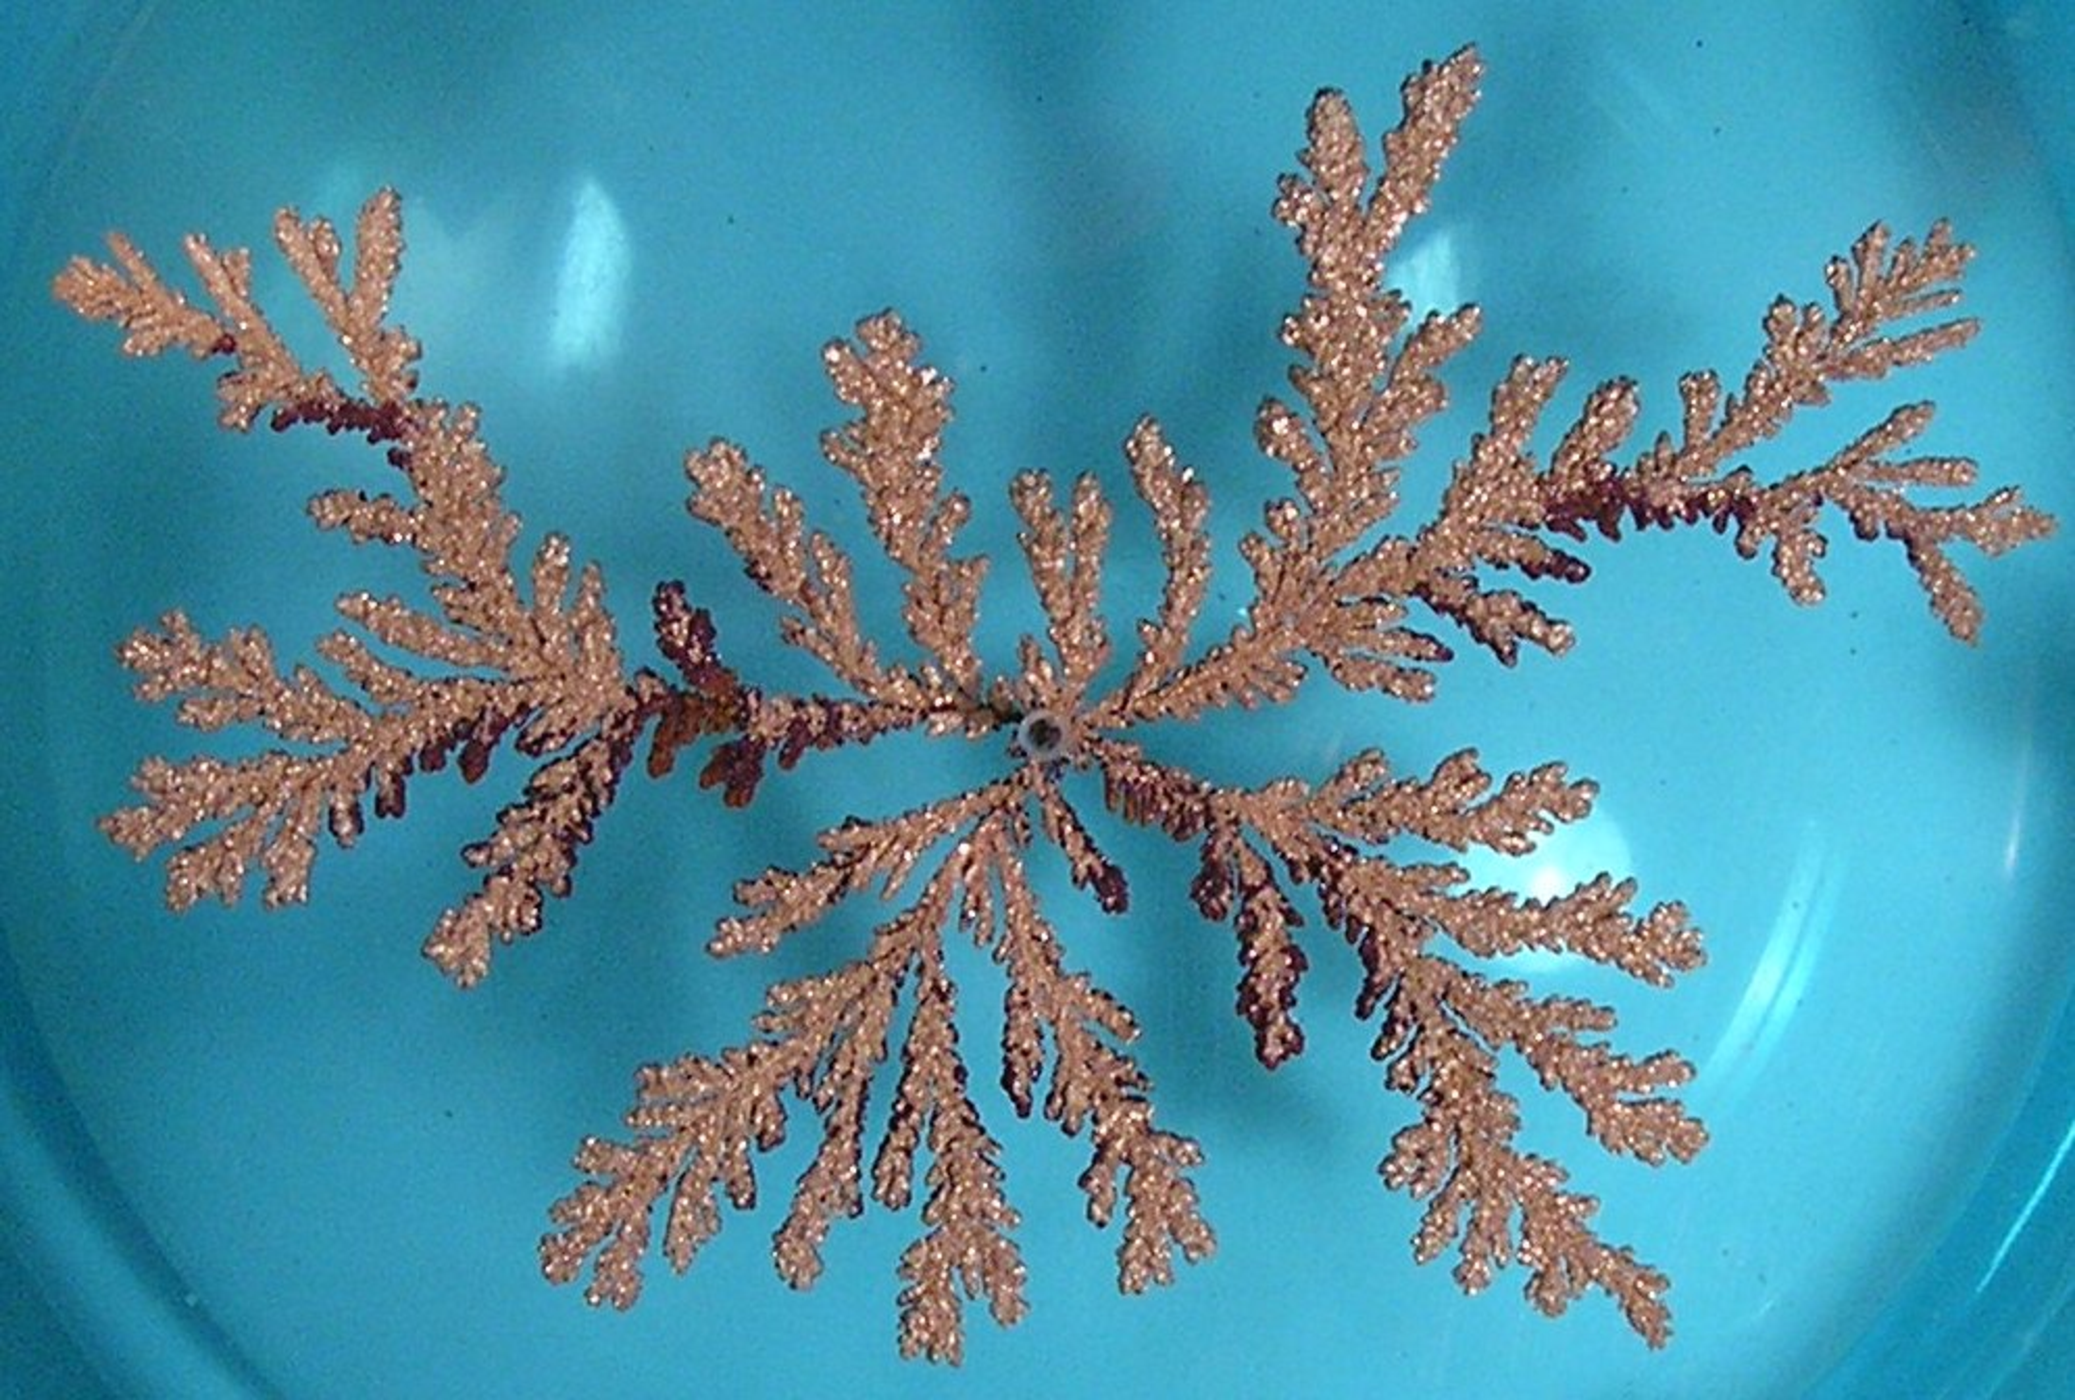
\includegraphics[width=2.5in]{16.Random-Walk/dla_experiment.pdf}}
		\caption{Electrodeposition of copper ions (Experiment)}
		\label{fig:dla_experiment}
	\end{subfigure}
	\begin{subfigure}{0.45\textwidth}
		\centering	
		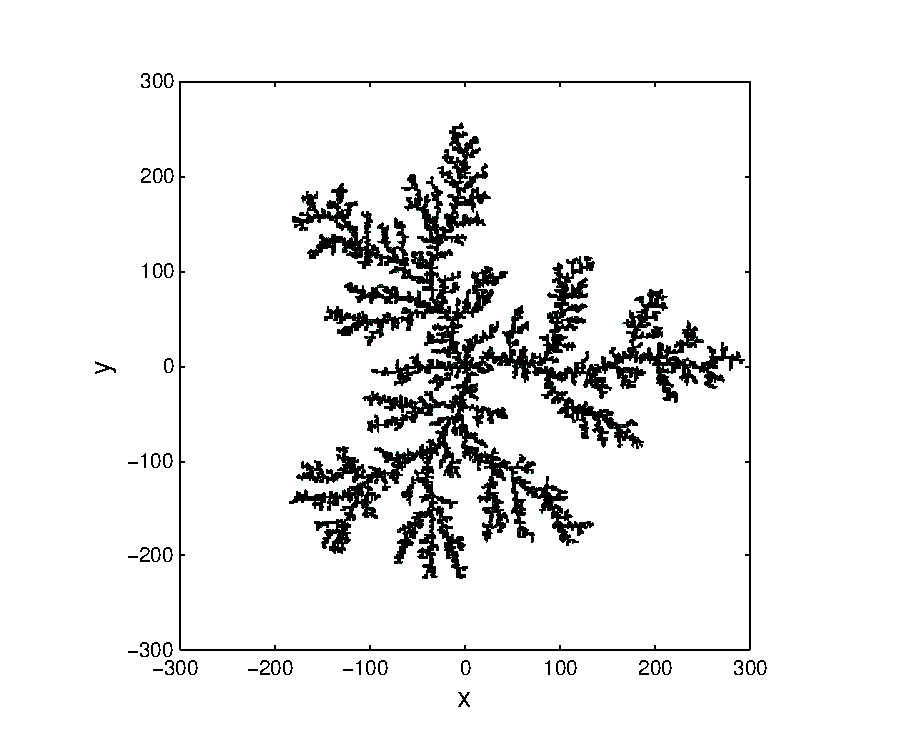
\includegraphics[width=2.5in]{16.Random-Walk/dla-simulation.pdf}	
		\caption{Simulation of DLA.  The cluster is formed with 20000 particles.}
		\label{fig:dla_simulation}
	\end{subfigure}
	\caption{Diffusion limited aggregates (DLA)}\label{fig:dla}
\end{figure}

\begin{figure}
	\centering
	\begin{subfigure}{0.45\textwidth}
		\centering
		\raisebox{5mm}{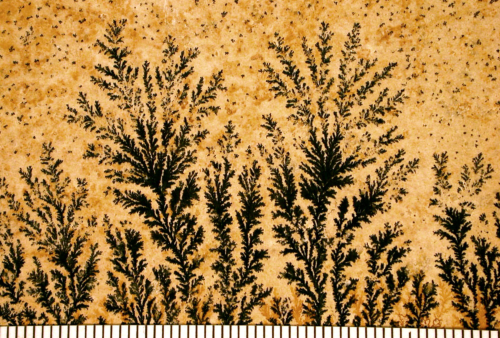
\includegraphics[width=2.5in]{16.Random-Walk/dendrites.pdf}}
		\caption{Manganese dendrites on a limestone.}
		\label{fig:dendrites_real}
	\end{subfigure}
	\begin{subfigure}{0.45\textwidth}
		\centering
		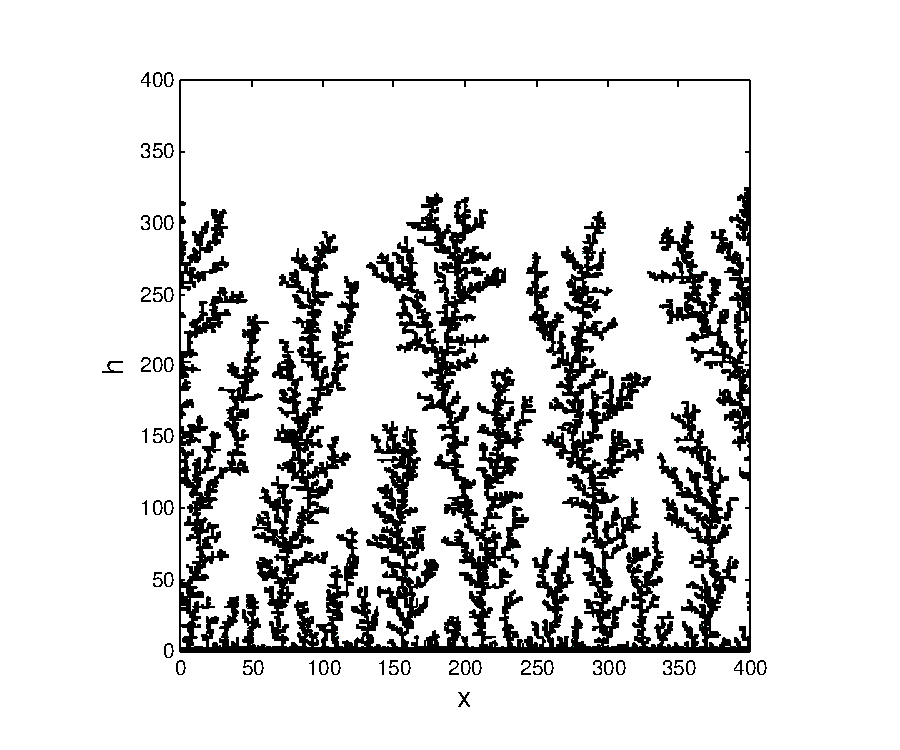
\includegraphics[width=2.5in]{16.Random-Walk/dendrites_simulation.pdf}	
		\caption{Simulation of dendrite growth.  The dendrites are formed with 10000 particles.}
		\label{fig:dendrites_simulation}
	\end{subfigure}
	\caption{Dendrite Crystals}\label{fig:dendrites}
\end{figure}



\newpage
\noindent
\subsection{Parrondo Paradox}

Suppose that you play games at a Casino.  Except for a few very lucky people, most of us lose and the Casino wins. In 1996, Juan Parrondo discovered an interesting paradox which states 

\bigskip
\begin{minipage}{6in}
\textit{There exist pairs of games, each with a higher probability of losing than winning, for which it is possible to construct a winning strategy by playing the games alternately.}
\end{minipage}

Algorithm \ref{alg:parrondo-game} is based on the original games invented by Parrondo.\cite{parrondo-game}

\begin{myalgobox}
\Algorithm{Parrondo Game}

\medskip
\begin{minipage}{5.5in}
\begin{enumerate}
\item   Winning a game earns us \$1 and losing requires us to surrender \$1. Let $C(t)$ be your capital at time $t$.  It follows that $C(t+1) = C(t) \pm 1$ after each play.
\item  In Game A, we toss a biased coin, Coin 1, with probability of winning $P_1=(1/2)-\epsilon$. If $\epsilon > 0$, this is clearly a losing game in the long run.
\item   In Game B, we first determine if our capital is a multiple of 3. If it is, we toss a biased coin, Coin 2, with probability of winning $P_2=(1/10)-\epsilon$. If it is not, we toss another biased coin, Coin 3, with probability of winning $P_3=(3/4)-\epsilon$. 
\end{enumerate}
\end{minipage}
\end{myalgobox}

\bigskip
When $\epsilon=0$, both Game A and B are fair and on average you neither lose or gain.  Game A is a simple biased random walk.  The Game B is similar to the persistent random walk since the jump probability depends on the additional degree of freedom.  Th idea behind this game came from a flashing ratchet model of biological molecular motors.\cite{ratchet-sciam,ratchet-phystoday}  However, if $\epsilon>0$, there is bias in each Game in favor of the Casino. 
In Program \ref{prog:parrondo}, the Parrondo game is implemented.
Figure \ref{fig:parrondo} shows capital gain for three different cases.  If you play Game A or Game B alone, you lose your money on average.  However, you gain if both games are played in the order of $AABBAABBAABB\cdots$.

\begin{figure}
\centering
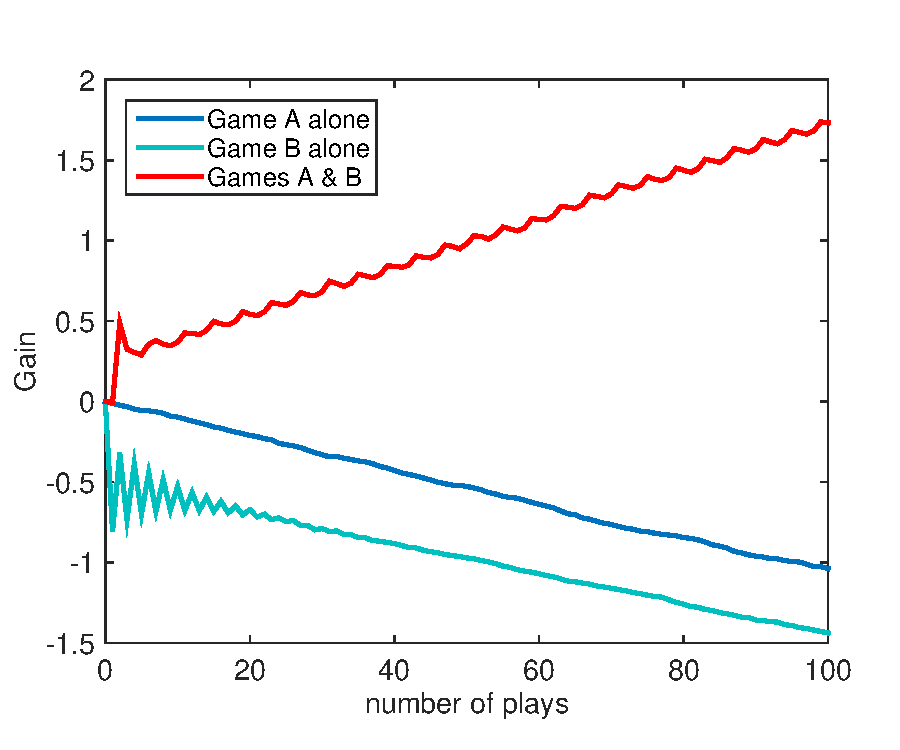
\includegraphics[width=2.5in]{16.Random-Walk/parrondo.pdf}
\caption{Simulation of Parrondo Game. 50000 people played Games in a Casino. When they play only Game A, on average people lose their money.  Similarly, only Game B is played, again on average people lose their money. Now  they play Game A for several times and switch to Game B. After playing Game B for several times switch back to Game A.  Then, repeat this many times. You always win!}
\label{fig:parrondo}
\end{figure}

\newpage
\noindent
\section{Problems}

\begin{enumerate}[labelwidth=0.5cm,labelindent=0cm,leftmargin=*,label=\bfseries \thechapter.\arabic*,align=left]

\item
The skewness and the kurtosis are defined by
\begin{equation}
\gamma_1 = \frac{\expval{(x-\mu)^3}}{\sigma^3}, \qquad \beta_2 = \frac{\expval{(x-\mu)^4}}{\sigma^4},
\end{equation}
respectively, where $\mu=\expval{x}$ and $\sigma^2=\expval{(x-\mu)^2}$.
The Gaussian distribution is uniquely determined by the mean and variance.  Higher order cumulants are all expressed with the mean and the variance.  For example,$\gamma_1=0$ and $\beta_2=3$.
Now, consider simple one-dimensional discrete random walk.  All particles are initially at $x=0$.  Find the distribution of particles after $N=1000$ steps.  Then, evaluate skewness and kurtosis.  Compare them with the exact values.   In order to get a reasonable agreement, you need to have a large number of particles.

\item Consider two-dimensional random walks discussed in Example \ref{ex:2d-rw}.   Find the time (number of steps) when the random walkers reach the circle of radius $r=30$ for the first time.  The time is also a stochastic variable which has a certain probability distribution.  Find the distribution and find the expectation value of the time, which is known as first passage time.

\item  Is the Parrondo paradox still valid when Games A or B is randomly chosen at every play with equal probability?  Modify Program \ref{prog:parrondo} and check if you still win.

\item Find the fractal dimension $D$ in Eq. \eqref{eq:dla-fractal-dimension} for the two-dimensional diffusion limited aggregates.

\end{enumerate}


\newpage
\noindent
\section*{MATLAB Source Codes}
\addcontentsline{toc}{section}{\protect\numberline{}MATLAB Source Codes}


\noindent
\program
\label{prog:rw_1d}
\footnotesize
\begin{lstlisting}[language=matlab]
%**************************************************************************
%*     Exercise 16.1                                                      *
%*     filename: ch16pr01.m                                               *
%*     program listing number: 16.1                                       *
%*                                                                        *
%*     This program simulates the one-dimensional descrete random walk.   *
%*                                                                        *
%*     Programed by Ryoichi Kawai for Computational Physics Course.       *
%*     Last modification:  03/03/2017.                                    *
%**************************************************************************
clear all

N=1000; % max time (number of steps)
M=100000; % number of particles

x=zeros(M,N); % reset the trajectories

% trajectory calculation
for i=1:N-1
    x(:,i+1)=x(:,i)+randi(2,[M,1])*2-3;
end

% stattistics
mu=sum(x,1)/M;  % mean
sigma=sqrt(sum(x.^2,1)/M);  %variance
t=[1:N];

subplot(1,2,1)
p=plot(t,mu,t,sigma,'--',t,-sigma,'--');
set(p(1),'color','red','linewidth',2)
set(p(2:3),'color','black','linewidth',2)
legend('\mu','+\sigma','-\sigma')
legend('location','northwest')
hold on
p=plot(t,x(1,:),t,x(2,:),t,x(3,:));
set(p(1),'color','blue');
set(p(2),'color','green');
set(p(3),'color',[0,0.75,0.75]);
axis([0 N -40 40])
xlabel('steps','fontsize',14)
ylabel('x','fontsize',14)
hold off

subplot(1,2,2)
rho=x(:,N);
h=histogram(rho,51,'Normalization','pdf');
hold on
X=h.BinEdges;
Y=1./sqrt(2*pi*N)*exp(-X.^2/(2.*N));
p=plot(X,Y);
set(p,'color','red','linewidth',2);
xlabel('x')
ylabel(texlabel('rho(x)'))
hold off
\end{lstlisting}
\normalsize

\noindent
\program
\label{prog:rw_1d_persistent}
\footnotesize
\begin{lstlisting}[language=matlab]
%**************************************************************************
%*     Exercise 16.2                                                      *
%*     filename: ch16pr02.m                                               *
%*     program listing number: 16.2                                       *
%*                                                                        *
%*     This program simulates the one-dimensional persistent random walk. *
%*                                                                        *
%*     Programed by Ryoichi Kawai for Computational Physics Course.       *
%*     Last modification:  03/04/2017.                                    *
%**************************************************************************
clear all;

% parameters
p=0.75;  % persistent jump probability
M=100000; % number of particles
N=1000; % number of steps

% initial states
x=zeros(M,1);
mu=zeros(N,1);
sigma2=zeros(N,1);
mu(1)=0.;
sigma2(1)=0.;

d=randi(2,[M,1])*2-3; %unbiased initial jump
x=x+d;
mu(2)=sum(x)/M;  % mean
sigma2(2)=sum(x.^2)/M-mu(2)^2; %variance

for i=3:N
    r=rand(M,1);
    k=r>p;  % direction is reversed.
    d(k)=-d(k);
    x=x+sign(d);  % jump
    mu(i)=sum(x)/M;  % mean
    sigma2(i)=sum(x.^2)/M-mu(i)^2; %variance
end

subplot(1,2,1)
p=plot([1:N],mu,[1:N],sigma2);
set(p(1),'linewidth',2,'color','blue')
set(p(2),'linewidth',2,'color','red')
hold on
p=plot([1:N],[1:N],'--');
set(p,'color','black')
legend('\mu','\sigma^2','\sigma^2 (Normal RW)')
legend('location','northwest')
xlabel('steps')
ylabel('moments')
hold off

subplot(1,2,2)
h=histogram(x,51,'Normalization','pdf');
y=h.BinEdges;
g=1.0/sqrt(2*pi*N)*exp(-y.^2/(2.0*N));
hold on
r=plot(y,g);
set(r,'color','red')
xlabel('x')
ylabel('probability density')
legend('persistent RW','normal RW')
hold off
\end{lstlisting}
\normalsize

\noindent
\program
\label{prog:rw_2d}
\footnotesize
\begin{lstlisting}[language=matlab]
%**************************************************************************
%*     Exercise 16.3                                                      *
%*     filename: ch16pr03.m                                               *
%*     program listing number: 16.3                                       *
%*                                                                        *
%*     This program simulates the two-dimensional random walk.            *
%*                                                                        *
%*     Programed by Ryoichi Kawai for Computational Physics Course.       *
%*     Last modification:  03/04/2017.                                    *
%**************************************************************************
clear all
close all

M=100000;  % number of Brownian particles

N=1000;    % number of steps

x=zeros(M,1);  % initial position
y=zeros(M,1);
u=zeros(N,2);
w=zeros(N,2);
s=zeros(N);

for i=2:N
    g=randi([1,4],[M,1]);  % pick one of four directions to jump
    
    x(g==1)=x(g==1)+1;
    x(g==2)=x(g==2)-1;
    y(g==3)=y(g==3)+1;
    y(g==4)=y(g==4)-1;
        
    % record two sample trajectories
    u(i,1)=x(1);
    w(i,1)=y(1);
    u(i,2)=x(2);
    w(i,2)=y(2);

    % mean square displacenent
    s(i)=sum(x.^2+y.^2)/M;
end

plot(u(:,1),w(:,1),u(:,2),w(:,2));
hold on
R=sqrt(s(N));
viscircles([0,0],R,'Color','r');
axis equal

L=R*1.5;
axis([-L L -L L])
xlabel('x','fontsize',14)
ylabel('y','fontsize',14)
hold off

figure
plot(x(1:2000),y(1:2000),'.');
axis equal; % fix the aspect ratio (needed for movie)
axis([-100 100 -100 100]);  % fiz the axis range
hold on
viscircles([0,0],R,'Color','r');
xlabel('x','fontsize',14)
ylabel('y','fontsize',14)
hold off
\end{lstlisting}
\normalsize

\noindent
\program
\label{prog:dla}
\footnotesize
\begin{lstlisting}[language=matlab]
%**************************************************************************
%*     Section 16.4.1                                                     *
%*     filename: ch16pr04.m                                               *
%*     program listing number: 16.4                                       *
%*                                                                        *
%*     This program simulates the two-dimensional diffusion limited       *
%*     aggregates.                                                        *
%*                                                                        *
%*     Programed by Ryoichi Kawai for Computational Physics Course.       *
%*     Last modification:  03/04/2017.                                    *
%**************************************************************************
clear all
close all

% number of particles
N=20000;

L=601;  % size of the square space
L0=301; % center of the square

% set array size
x=zeros(N,1);
y=zeros(N,1);
A=zeros(L,L);

R=5;         % inner circle
R_max=3*R;   % outer circle

% seed particle
A(L0,L0)=1;
x(1)=L0;
y(1)=L0;
viscircles([x(1),y(1)],0.5,'Color','r');
axis equal
hold on

for n=2:N
    % random point on the inner circle
    theta=rand(1)*2*pi;
    x(n)=round(R*cos(theta))+L0;
    y(n)=round(R*sin(theta))+L0;
    
    % diffusion
    found=false; 
    while not(found)
        p=rand(1);
        if p<1/4
            x(n)=x(n)+1;
        elseif p<1/2
            x(n)=x(n)-1;
        elseif p<3/4
            y(n)=y(n)+1;
        else
            y(n)=y(n)-1;
        end
        r=sqrt((x(n)-L0)^2+(y(n)-L0)^2);
        if r>R_max  % out of bound - restart
            theta=rand(1)*2*pi;
            x(n)=round(R*cos(theta))+L0;
            y(n)=round(R*sin(theta))+L0;
        elseif r<R
            % hit the cluster?
            if A(x(n)+1,y(n))+A(x(n)-1,y(n))...
              +A(x(n),y(n)+1)+A(x(n),y(n)-1)>0
                found=true;
                A(x(n),y(n))=1;
                viscircles([x(n),y(n)],0.5,'Color','r');
                drawnow
                R = max(R, r+5); % adjust inner circle radius
                R_max = 3*R;     % adjust outer circle radius
                if R>L0
                    xlabel('x','fontsize',14)
                    ylabel('y','fontsize',14)
                    hold off
                    error('Out of Range')
                end
            end
        end
    end
end
\end{lstlisting}
\normalsize

\noindent
\program
\label{prog:dendrite}
\footnotesize
\begin{lstlisting}[language=matlab]
%**************************************************************************
%*     Section 16.4.2                                                     *
%*     filename: ch16pr05.m                                               *
%*     program listing number: 16.5                                       *
%*                                                                        *
%*     This program simulates the growth of dendrite.                     *
%*                                                                        *
%*     Programed by Ryoichi Kawai for Computational Physics Course.       *
%*     Last modification:  03/04/2017.                                    *
%**************************************************************************
clear all
close all

% size of the systrem
N=5000;
Lx=100;
Ly=100;

% initial setting
x=zeros(N,1);
y=zeros(N,1);
A=zeros(Lx,2*Ly);
A(:,1)=1;
H=5;
ymax=5;

% bias in y direction
e=0.01;

% initial plots
p=plot([0,Lx-1],[0.5,0.5]);
set(p,'linewidth',2,'color','black')
axis equal
axis([0 Lx 0 100])
hold on

% random position
x=floor(rand(N,1)*Lx);

% deposition process
for n=1:N
    y(n)=H;  % diffusion starts from here 
    
    found=false;
    
    % diffues in 2D space until it sticks to another.
    while not(found)
        p=rand(1);
        if p<1/4
            x(n)=mod(x(n)+1,Lx);
        elseif p<1/2
            x(n)=mod(x(n)-1,Lx);
        elseif p<3/4-e
            y(n)=y(n)+1;
            if y(n)>3*H  % if it went to high, start over.
               y(n)=H;
            end
        else
            y(n)=y(n)-1;
        end
        
        if y(n)<H
            i1=mod(x(n)-1,Lx)+1; 
            i2=mod(x(n)+1,Lx)+1;
            if A(i1,y(n)+1)+A(i2,y(n)+1)...
              +A(x(n)+1,y(n)+2)+A(x(n)+1,y(n))>0
                found=true;
                A(x(n)+1,y(n)+1)=1;
                viscircles([x(n)+1,y(n)+1],0.5,'Color','b');
                drawnow
                ymax=max(y(n),ymax); % adjust the stating height
                H=5+ymax;
                if ymax>Ly-1
                    axis([0 Lx 0 ymax*1.1])
                    xlabel('x','fontsize',14)
                    ylabel('y','fontsize',14)
                    hold off
                    error('Out of Range')
                end
            end
        end
    end
end
\end{lstlisting}
\normalsize

\noindent
\program
\label{prog:parrondo}
\footnotesize
\begin{lstlisting}[language=matlab]
%**************************************************************************
%*     Section 16.4.3                                                     *
%*     filename: ch16pr06.m                                               *
%*     program listing number: 16.6                                       *
%*                                                                        *
%*     This program simulates the Parrondo game.                          *
%*                                                                        *
%*     Programed by Ryoichi Kawai for Computational Physics Course.       *
%*     Last modification:  03/04/2017.                                    *
%**************************************************************************
clear all
close all

% control parameters
e=0.005;
pA=1/2-e;
qA=1-pA;
pB=3/4-e;
qB=1-pB;
pC=1/10-e;
qC=1-pC;
N=50000;
M=100;

% Game A
x=zeros(N,1);
y=zeros(M+1,1);
for i=1:M
    r=rand(N,1);
    x(r<pA)=x(r<pA)+1;
    x(r>=pA)=x(r>=pA)-1;    
    y(i+1)=sum(x)/N;
end

p=plot([0:M],y);
set(p,'linewidth',2)
hold on

% Game B
x=zeros(N,1);
p=zeros(N,1);
for i=1:M
    r=rand(N,1);
    p(:)=pB;
    k=find(mod(x,3)==0);
    p(k)=pC;
    x(r<p)=x(r<p)+1;
    x(r>=p)=x(r>=p)-1;  
    y(i+1)=sum(x,1)/N;
end
p=plot([0:M],y);
set(p,'linewidth',2,'color',[0, 0.75,0.75])
hold on

% Game A and B
x=zeros(N,1);
p=zeros(N,1);
for i=1:M
    r=rand(N,1);
    if mod(i,4)<2
        p(:)=pA;
    else
        p(:)=pB;
        k=find(mod(x,3)==0);
        p(k)=pC;
    end
    x(r<p)=x(r<p)+1;
    x(r>=p)=x(r>=p)-1;  
    y(i+1)=sum(x,1)/N;
end
p=plot([0:M],y);
set(p,'linewidth',2,'color','red')
legend('Game A alone','Game B alone', 'Games A & B')
legend('location','northwest')
xlabel('# of plays','fontsize',14)
ylabel('Gain','fontsize',14)
hold off
\end{lstlisting}
\normalsize

\bigskip
\noindent
\section*{Python Source Codes}
\addcontentsline{toc}{section}{\protect\numberline{}Python Source Codes}
\setcounter{program}{0}

\bigskip
\noindent
\program
\footnotesize
\begin{lstlisting}[language=python]
#!/usr/bin/env python3
# -*- coding: utf-8 -*-
"""
%**************************************************************************
%*     Exercise 16.1                                                      *
%*     filename: ch16pr01.py                                              *
%*     program listing number: 16.1                                       *
%*                                                                        *
%*     This program simulates the one-dimensional descrete random walk.   *
%*                                                                        *
%*     Programed by Ryoichi Kawai for Computational Physics Course.       *
%*     Last modification:  02/15/2014.                                    *
%**************************************************************************
"""
import numpy as np
import matplotlib.pyplot as plt

N=1000    # max time (number of steps)
M=100000  # number of particles

x=np.zeros((M,N+1))  # reset the trajectories

# trajectory calculation
for i in range(0,N):
    x[:,i+1]=x[:,i]+np.random.choice([-1,1],M) # random step

# stattistics
mu=np.sum(x,axis=0)/M        # mean
sigma=np.sqrt(np.sum(x**2,axis=0)/M)-mu**2  #variance
t=np.linspace(0,N,N+1)

plt.figure(figsize=(12,5))
plt.subplot(1,2,1)
plt.plot(t,mu,'-r',label=r'$\mu$')
plt.plot(t, sigma,'--k',label=r'$+\sigma$')
plt.plot(t,-sigma,'--k',label=r'$-\sigma$')
plt.plot(t,x[0,:],'-b')
plt.plot(t,x[1,:],'-g')
plt.plot(t,x[2,:],'-c')
plt.axis([0, N, -40, 40])
plt.xlabel('steps',fontsize=14)
plt.ylabel('x',fontsize=14)
plt.legend(loc=3)

plt.subplot(1,2,2)
rho=x[:,N]
n, X, Y = plt.hist(rho,51,normed=True,label='simulation')
Y=1.0/np.sqrt(2*np.pi*N)*np.exp(-X**2/(2.*N))
dX=X[2]-X[1]
plt.plot(X,Y,'-r',label='theory')
plt.xlabel('x')
plt.ylabel(r'$\rho(x)$')
plt.legend(loc=1)
plt.show()
\end{lstlisting}
\normalsize

\bigskip
\noindent
\program
\footnotesize
\begin{lstlisting}[language=python]
#!/usr/bin/env python3
# -*- coding: utf-8 -*-
"""
%**************************************************************************
%*     Exercise 16.2                                                      *
%*     filename: ch16pr02.m                                               *
%*     program listing number: 16.2                                       *
%*                                                                        *
%*     This program simulates the one-dimensional persistent random walk. *
%*                                                                        *
%*     Programed by Ryoichi Kawai for Computational Physics Course.       *
%*     Last modification:  03/04/2017.                                    *
%**************************************************************************
"""
import numpy as np
import matplotlib.pyplot as plt

# parameters
p=0.75   # persistent jump probability
M=100000  # number of particles
N=1000    # number of steps

mu=np.zeros(N+1)
sigma2=np.zeros(N+1)
t=np.linspace(0,N,N+1)

# initial states
x=np.zeros(M)  # reset the trajectories
mu[0]=0.
sigma2[0]=0.

d=np.random.choice([-1,1],M)
x=x+d # unbiased initial jump
mu[1]=np.sum(x)/M        # mean
sigma2[1]=np.sum(x**2)/M-mu[1]**2  #variance

for i in range(1,N+1):
    r=np.random.rand(M)
    k=r>p  # direction is reversed.
    d[k]=-d[k]
    x=x+np.sign(d)        # jump
    mu[i]=np.sum(x)/M;       # mean
    sigma2[i]=np.sum(x**2)/M  # ariance

plt.figure(figsize=(12,5))
plt.subplot(1,2,1)
plt.plot(t,mu,'-b',label=r'$\mu$',linewidth=2)
plt.plot(t,sigma2,'-r',label=r'$\sigma^2$',linewidth=2)
plt.plot(t,t,'--k',label='$\sigma^2$ (Normal RW)')
plt.legend(loc=2)
plt.xlabel('steps')
plt.ylabel('moments')

plt.subplot(1,2,2)
n, X, Y = plt.hist(x,51,normed=True,label='persistent RW')
dX=X[2]-X[1]
Z=1.0/np.sqrt(2.0*np.pi*N)*np.exp(-X**2/(2.0*N))
plt.plot(X,Z,'-r',label='normal RW')
plt.xlabel('x')
plt.ylabel('probability distribution')
plt.legend(loc=1)
plt.show()
\end{lstlisting}
\normalsize

\bigskip
\noindent
\program
\footnotesize
\begin{lstlisting}[language=python]
#!/usr/bin/env python3
# -*- coding: utf-8 -*-
"""
%**************************************************************************
%*     Exercise 17.3                                                      *
%*     filename: ch17pr03.m                                               *
%*     program listing number: 17.3                                       *
%*                                                                        *
%*     This program simulates the two-dimensional random walk.            *
%*                                                                        *
%*     Programed by Ryoichi Kawai for Computational Physics Course.       *
%*     Last modification:  02/15/2014.                                    *
%**************************************************************************
"""
import numpy as np
import matplotlib.pyplot as plt

M=100000  # number of particles
N=1000    # number of steps

x=np.zeros(M)  # initial position
y=np.zeros(M)

u=np.zeros((N+1,2))
w=np.zeros((N+1,2))
s=np.zeros(N+1)

for i in range(1,N+1):

    g=np.random.random_integers(1,4,M)  # pick one of four directions to jump
    
    # jump
    # The following expression is easy to write but slow in execution
    x[g==1]+=1
    x[g==2]+=-1
    y[g==3]+=1
    y[g==4]+=-1
    
    # record two sample trajectories
    u[i,0]=x[0]
    w[i,0]=y[0]
    u[i,1]=x[1]
    w[i,1]=y[1]

    # mean square displacenent
    s[i]=sum(x**2+y**2)/M

fig1, ax=plt.subplots(figsize=(6,6))
plt.plot(u[:,0],w[:,0],'-b')
plt.plot(u[:,1],w[:,1],'-g')
R=np.sqrt(s[N])
c=plt.Circle((0, 0), R, color='r',fill=False)
ax.add_artist(c)
ax.axis('equal')
L=R*1.5
ax.axis([-L, L, -L, L])
plt.xlabel('x',fontsize=14)
plt.ylabel('y',fontsize=14)
plt.legend(loc=1)

fig2, bx=plt.subplots(figsize=(6,6))

plt.plot(x[0:2000],y[0:2000],'.')
c=plt.Circle((0, 0), R, color='r',fill=False,linewidth=2)
bx.add_artist(c)
bx.axis('equal') 
bx.axis([-100, 100, -100, 100]) 

plt.xlabel('x',fontsize=14)
plt.ylabel('y',fontsize=14)

plt.show()
\end{lstlisting}
\normalsize

\bigskip
\noindent
\program
\footnotesize
\begin{lstlisting}[language=python]
#!/usr/bin/env python3
# -*- coding: utf-8 -*-
"""
#**************************************************************************
#*     Section 16.4.1                                                     *
#*     filename: ch16pr04.py                                              *
#*     program listing number: 16.4                                       *
#*                                                                        *
#*     This program simulates the two-dimensional diffusion limited       *
#*     aggregates.                                                        *
#*                                                                        *
#*     Programed by Ryoichi Kawai for Computational Physics Course.       *
#*     Last modification:  03/04/2017.                                    *
#**************************************************************************
"""
import numpy as np
import matplotlib.pyplot as plt

anim=True

# number of particles
N=10000

L=601 # size of the square space
L0=np.int(L/2) # center of the square

# set array size
x=np.zeros(N,dtype=np.int)
y=np.zeros(N,dtype=np.int)
A=np.zeros((L,L),dtype=np.int)

R=5.         # inner circle
R_max=3.*R   # outer circle

# seed particle
A[L0,L0]=1
x[0]=L0
y[0]=L0

plt.ion()
fig, ax = plt.subplots(figsize=(8,8))
ax.set_xlim([L0-100,L0+100])
ax.set_ylim([L0-100,L0+100])

c=plt.Circle((x[0],y[0]), 0.5, color='b')
ax.add_artist(c)


for n in range(1,N):
    # random point on the inner circle
    theta=np.random.rand(1)*2.0*np.pi
    x[n]=np.int(R*np.cos(theta))+L0
    y[n]=np.int(R*np.sin(theta))+L0
    
    # diffusion
    found=False 
    while not(found):
        p=np.random.rand(1)
        if p<1./4.:
            x[n]+=1
        elif p<1./2.:
            x[n]+=-1
        elif p<3./4.:
            y[n]+=1
        else:
            y[n]+=-1

        r=np.sqrt(np.float((x[n]-L0)**2+(y[n]-L0)**2))
        if r>R_max:  # out of bound - restart
            theta=np.random.rand(1)*2.0*np.pi
            x[n]=np.int(R*np.cos(theta))+L0
            y[n]=np.int(R*np.sin(theta))+L0
        elif r<R:
            # hit the cluster?
            if A[x[n]+1,y[n]]+A[x[n]-1,y[n]]+A[x[n],y[n]+1]+A[x[n],y[n]-1]>0:
                found=True
                A[x[n],y[n]]=1
                c=plt.Circle((x[n],y[n]), 0.5, color='b',fill=False)
                ax.add_artist(c)
                if anim:
                    plt.pause(0.0001)
                if R<r+5:
                    R=r+5. # adjust inner circle radius
                R_max = 3*R     # adjust outer circle radius
                if R>L0:
                    plt.xlabel('x',fontsize=14)
                    plt.ylabel('y',fontsize=14)
                    plt.show()
                    exit('Out of Range')
\end{lstlisting}
\normalsize

\bigskip
\noindent
\program
\footnotesize
\begin{lstlisting}[language=python]
#!/usr/bin/env python3
# -*- coding: utf-8 -*-
"""
#**************************************************************************
#*     Section 17.4.2                                                     *
#*     filename: ch17pr05.m                                               *
#*     program listing number: 17.5                                       *
#*                                                                        *
#*     This program simulates the growth of dendrite.                     *
#*                                                                        *
#*     Programed by Ryoichi Kawai for Computational Physics Course.       *
#*     Last modification:  02/15/2014.                                    *
#**************************************************************************
"""
import numpy as np
import matplotlib.pyplot as plt

anim=True

# size of the systrem
N=5000 
Lx=100 
Ly=100 

plt.ion()
fig, ax = plt.subplots(figsize=(6,6))
plt.axis('equal')
ax.set_xlim([0,Lx])
ax.set_ylim([0,Ly])

# initial setting
x=np.random.random_integers(0,Lx-1,N)  #  horizontal position (uniform random)
y=np.zeros(N,dtype=np.int) 
A=np.zeros((Lx,2*Ly),dtype=np.int) 
A[:,0]=1 
H=5 
ymax=5 

# bias in y direction
e=0.01 

# initial plots
plt.plot([0,Lx-1],[0.5,0.5],'-k',linewidth=2) 

# deposition process
for n in range(0,N):
    y[n]=H   # diffusion starts from here 
    
    found=False 
    
    # diffues in 2D space until it sticks to another.
    while not(found):
        p=np.random.rand(1) 
        if p<1./4.:
            x[n]=np.mod(x[n]+1,Lx)   # periodic boundary
        elif p<1./2.:
            x[n]=np.mod(x[n]-1,Lx)   # periodic boundary
        elif p<3./4.-e:  
            y[n]=y[n]+1 
            if y[n]>3*H:  # if it went to high, start over.
               y[n]=H 
        else:
            y[n]=y[n]-1 

        if y[n]<H:
            i1=np.mod(x[n]-1,Lx) 
            i2=np.mod(x[n]+1,Lx) 
            if A[i1,y[n]]+A[i2,y[n]]+A[x[n],y[n]+1]+A[x[n],y[n]-1]>0:
                found=True 
                A[x[n],y[n]]=1 
                c=plt.Circle((x[n],y[n]), 0.5, color='b',fill=False)
                ax.add_artist(c)
                if anim:
                    plt.pause(0.0001)

                ymax=np.max([y[n],ymax])  # adjust the stating height
                H=5+ymax 
                if ymax>Ly-1:
                    plt.xlabel('x',fontsize=14)
                    plt.ylabel('y',fontsize=14)
                    plt.show()
                    exit('Out of Range')
\end{lstlisting}
\normalsize

\bigskip
\noindent
\program
\footnotesize
\begin{lstlisting}[language=python]
#!/usr/bin/env python3
# -*- coding: utf-8 -*-
"""
#**************************************************************************
#*     Section 16.4.3                                                     *
#*     filename: ch16pr06.py                                              *
#*     program listing number: 16.6                                       *
#*                                                                        *
#*     This program simulates the Parrondo game.                          *
#*                                                                        *
#*     Programed by Ryoichi Kawai for Computational Physics Course.       *
#*     Last modification:  03/04/2017.                                    *
#**************************************************************************
"""
import numpy as np
import matplotlib.pyplot as plt

# control parameters
e=0.005
pA=1./2.-e
qA=1.-pA
pB=3./4.-e
qB=1.-pB
pC=1./10.-e
qC=1.-pC
N=50000
M=100

# Game A
x=np.zeros(N)
y=np.zeros(M+1)
t=np.linspace(0,M,M+1)
for i in range(1,M+1):
    r=np.random.rand(N)
    x[r<pA]=x[r<pA]+1
    x[r>=pA]=x[r>=pA]-1
    y[i]=x.sum()/N

plt.figure(figsize=(6,5))
plt.plot(t,y,'-b',label='Game A alone',linewidth=2)

# Game B
x=np.zeros(N)
p=np.zeros(N)

for i in range(1,M+1):
    r=np.random.rand(N)
    p[:]=pB
    k=np.mod(x,3)==0
    p[k]=pC
    x[r<p]=x[r<p]+1
    x[r>=p]=x[r>=p]-1
    y[i]=x.sum()/N

plt.plot(t,y,'-g',label='Game B alone',linewidth=2)

# Alternating Game A and B
x=np.zeros(N)
p=np.zeros(N)

for i in range(1,M+1):
    r=np.random.rand(N)
    if np.mod(i,4)<2:
        p[:]=pA
    else:
        p[:]=pB
        k=np.mod(x,3)==0
        p[k]=pC

    x[r<p]=x[r<p]+1
    x[r>=p]=x[r>=p]-1
    y[i]=x.sum()/N

plt.plot(t,y,'-r',label='Game A & B',linewidth=2)

plt.legend(loc=2)
plt.xlabel('# of plays',fontsize=14)
plt.ylabel('Gain',fontsize=14)
plt.show()
\end{lstlisting}
\normalsize



\vfill

\newpage
%\chapbibliography
\bibliographystyle{unsrt}
\bibliography{compphys}
